\subsection{Felhasznált főbb könyvtárak}

\begin{itemize}
  \item \textbf{React}: A központi állapot nézetté történő leképezésére, a HTML
  elemek fölött használt állapottal rendelkező komponensek absztrakciójának
  megteremtésére. (A hagyományos MVC architektúrában leginkább a view szerepét
  tölti be.) \\
  https://reactjs.org/

  \item \textbf{Redux}: Az alkalmazás központi állapotának tárolásához és
  kezeléséhez. (A tradicionális MVC architektúrából leginkább a modell és a
  kontroller kombinációjának feleltethető meg.) \\
  https://redux.js.org/

  \item \textbf{OpenLayers}: Az interaktív térkép és a rajta megjelenő
  objektumok kirajzolásához. \\
  https://openlayers.org/

  \item \textbf{ol-react}: Az OpenLayers könyvtár által nyújtott funkciók React
  komponensekként való kezeléséhez. \\
  https://www.npmjs.com/package/ol-react

  \item \textbf{Golden Layout}: A dinamikus, felhasználó által személyre szabható
  felület kialakítására. \\
  https://golden-layout.com/

  \item \textbf{Material UI}: A felhasználói felületen megjelenő elemek
  kinézetéhez. \\
  http://www.material-ui.com/ | https://material-ui-next.com/

  \item \textbf{mini-signals}: Az alkalmazás komponensei közötti üzenetküldésre.
  \\
  https://github.com/Hypercubed/mini-signals

  \item \textbf{Electron}: Az önállóan futtatható becsomagolt állomány
  létrehozásához. \\
  https://electronjs.org/
\end{itemize}

\section{Háttér modell}

\subsection{A Redux működése}

Mint az már korábban említésre került, a modell és a kontroller szerepét
egyaránt a Redux csomag tölti be. Ennek működése azon alapul, hogy a háttérben
több kisebb független modell összekapcsolásával jön létre egy összetettebb
állapot, melynek a frissebb állapotra cserélése kizárólag előre megadott akciók
segítségével történik, így garantálva a konzisztenciát.

A Redux alapon működő React megjelenítési réteget használó alkalmazások egyfajta
állandó körforgást valósítanak meg, amit az alábbi kép (\ref{fig:redux_react}.
ábra) szemléltet. A folyamat egy kezdeti állapotból indul, amely alapján a
React komponensek elvégzik az első megjelenítést. Ezt követően a React
komponensek kezdeményezhetnek akciókat, amelyek segítségével a régi állapotból
az adott akcióhoz tartozó redukáló függvények létrehoznak egy új állapotot. Az
új állapot bekerül az állapottárba, onnan pedig továbbítódik a komponensek felé,
ezáltal, amennyiben szükséges, egy újrarajzolást kezdeményezve. A központi
állapotobjektum tehát soha nem mutálódik, ehelyett mindig egy új verzió készül
belőle. Így az egész folyamat felfogható úgy, hogy az aktuális állapot mindig
egy kezdeti állapotból és a rajta végrehajtott akciók sorozatából redukálva
kapható meg, a megjelenő felület pedig ennek az aktuális állapotnak a
leképeződése.

\begin{figure}[H]
  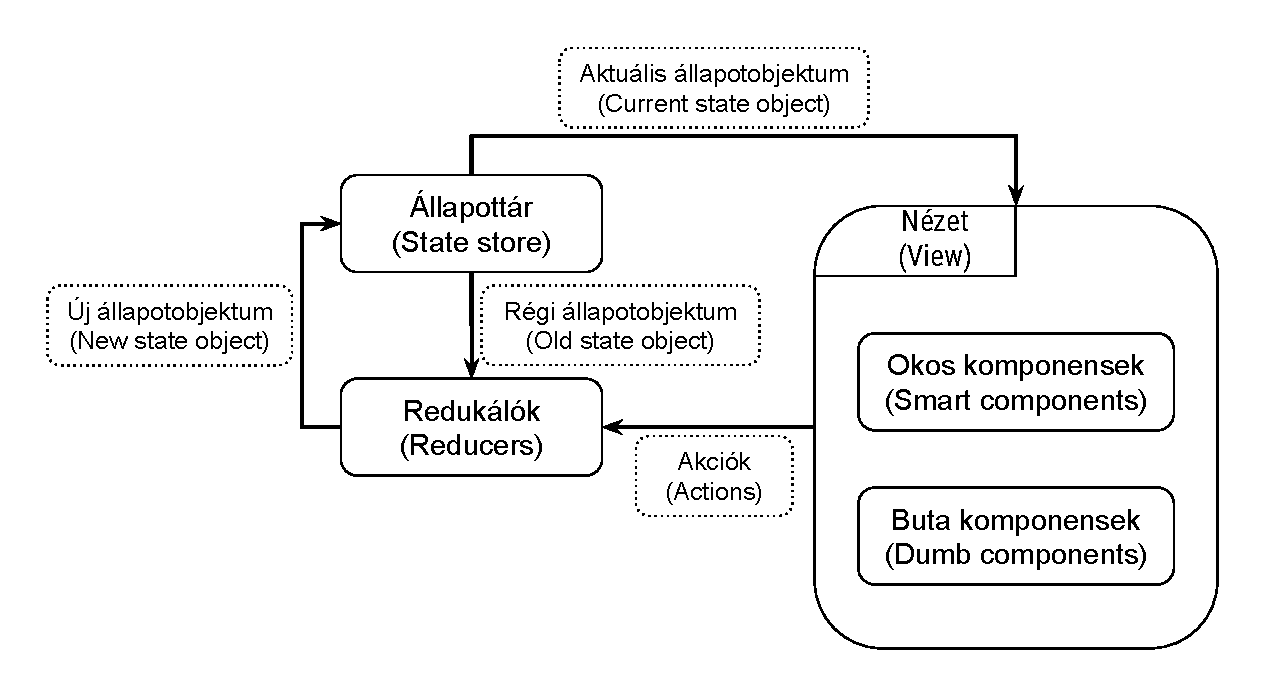
\includegraphics[width=\textwidth]{redux_react.pdf}
  \caption{A Redux és a React együttműködése}
  \label{fig:redux_react}
\end{figure}

A kép (\ref{fig:redux_react}. ábra) "Nézet" buborékon kívüli része tehát a Redux
folyamatait ábrázolja, a "Nézet" buborékon belül pedig a React-hez tartozó rész
látható. Azon belül találhatóak úgynevezett "okos" és "buta" komponensek. Ezek
között az tesz különbséget, hogy míg az "okos" komponensek tisztában vannak az
állapotobjektum szerkezetével, addig a "buta" komponenseknek már csak a
megjelenítéshez szükséges adatokat továbbítják.

\noindent Perzisztencia céljából a központi állapot bizonyos részei adott
időközönként automatikusan mentésre kerülnek a böngésző által felkínált
\verb|localStorage| API segítségével az alkalmazást futtató számítógépre, az
alkalmazás megnyitásakor pedig innen töltődnek be, így például a beállított
színezési predikátumok és a térkép elmentett állapotai megmaradnak az oldal
frissítése után is.
